\documentclass[12pt]{article}
\usepackage{cmbright}
\usepackage{amsmath}
\usepackage{bm}
\usepackage{graphicx}
\usepackage{enumitem}
\usepackage{tikz}
\usepackage[top=2.75cm, bottom=2.50cm, left=3.00cm, right=2.50cm]{geometry}
\usepackage{float}
\usepackage[binary-units=true]{siunitx}
\usepackage{xcolor}

\setlength{\headsep}{5pt}
\setlength\parindent{0pt}

\newlist{buttons}{itemize}{1}
\setlist[buttons,1]{}

\newcommand\norm[1]{\left\lVert#1\right\rVert}
\newcommand*\circled[2]{\tikz[baseline=(char.base)]{
    \node[shape=circle, draw={#2}, thick, inner sep=0.5pt] (char) {\textcolor{#2}{#1}};}}

\makeatletter
\renewcommand{\maketitle}{
      \bgroup\setlength{\parindent}{0pt}
      \begin{flushleft}
        \huge{\@title}\\
        \large{\@author}\\
        \rule{155pt}{0.4pt}
      \end{flushleft}\egroup
}
\makeatother

\title{NMR-EsPy}
\author{Simon Hulse\\ \texttt{simon.hulse@chem.ox.ac.uk}}
\date{}

\definecolor{myred}{HTML}{FE0000}
\definecolor{myblue}{HTML}{0005FF}
\definecolor{myorange}{HTML}{FE9A00}
\definecolor{mypurple}{HTML}{BA00FF}

\begin{document}
\maketitle
\section{Introduction}
NMR-EsPy is a program which attempts to estimate the parameters which describe an NMR signal. It is based on the assumption that a free induction decay (FID) is composed of a summation of damped sinusoidal oscillations, with experimental noise. Using this program, it is possible to perform a full spectral estimation, or consider only a specific region of interest. If the spectrum you are interested in has a high complexity, and you are only interested in a specific region, it is reccommended you specify this region, rather than performing a full estimation to drastically reduce the computational cost.

\section{Using the NMR-EsPy GUI}
After issuing the command \texttt{nmrespy} in TopSpin, the following window will appear:
\begin{figure}[H]
  \begin{center}
    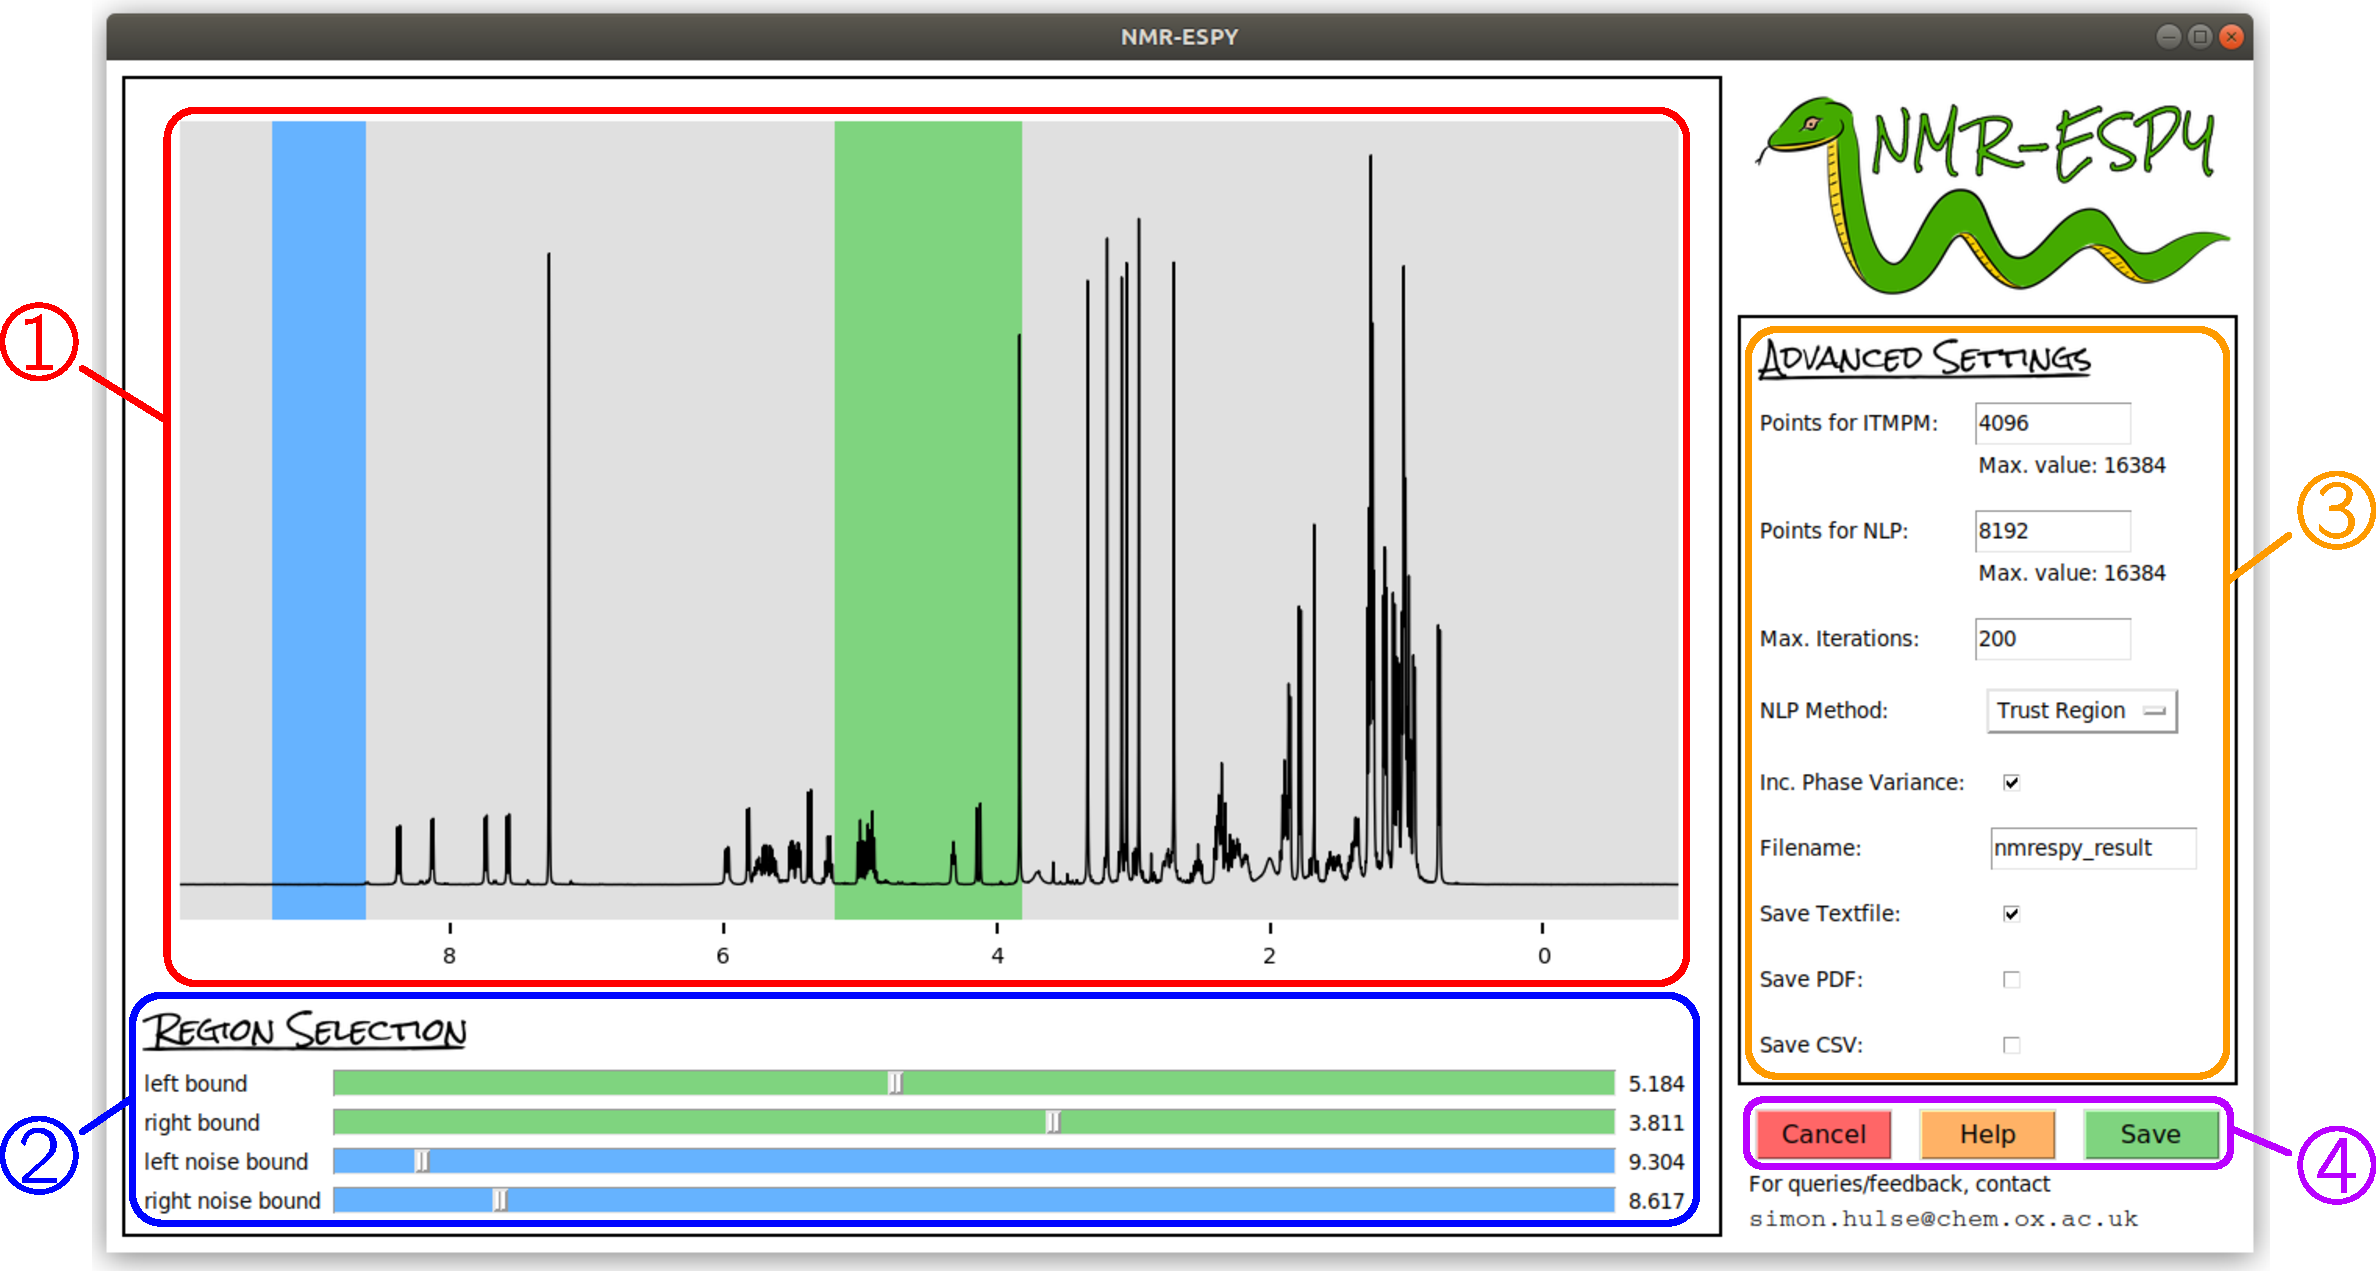
\includegraphics[scale=0.38]{./pictures/nmrespy_window.pdf}
  \end{center}
\end{figure}

\subsection{Part \textmd{\protect\circled{1}{myred}}: The Spectrum}
Here, the spectral data is plotted. You can nagivgate the plot in the following ways:
\begin{itemize}
  \item To zoom into a specific part of the spectrum, click and hold the left mouse button, drag the mouse, and finally release. The rectangle defined by this action will determine the new limits of the spectrum.
  \item To go back to the previous viewpoint, right click anywhere in the grey region.
  \item To go back to the original spectral view (i.e. the view of the entire spectrum), double right click anywhere in the grey region.
\end{itemize}

\subsection{Part \textmd{\protect\circled{2}{myblue}}: Region Selection}
Here, you may specify the spectral region you are interested in estimating. The region that will be estimated is given by the green region in the spectrum. As well as this, you will need to specify a section of the spectrum that does not contain any noticable peaks. This region is defined by the blue rectangle. The four slide bars in Region \circled{2}{myblue} allow you to change the boundaries of the two regions.

\subsection{Part \textmd{\protect\circled{3}{myorange}}: Advanced Settings}
Here, you may tweak various aspects of the estimation routine, as well as how the results are saved. Everything is this section is set to a default initially, and so it is not strictly necessary to alter these. The options that may be altered are as follows:
\begin{itemize}[leftmargin=*, label={}]
  \item \textbf{Points for ITMPM} Specifies the number of initial points in the time-domain signal to consider when the Matrix Pencil Method is performed. The default value is the number of points in the full signal, or 4096, whichever is smaller. In certain cases, it may be advisable to increase this value, though you will need decent amounts of RAM ($\SI{8}{\gibi\byte}$ or higher).
  \item \textbf{Points for NLP} Specifies the number of initial points in the time-domain signal to consider when nonlinear programming is performed. The default value is of points in the full signal, or 8192, whichever is smaller.
  \item \textbf{Max. Iterations} The maximum number of iterations the routine is allowed to perform before it is terminated. If this number of iterations is reached before convergence, the result at that moment is returned.
  \item \textbf{NLP Method} Specifies the nonlinear optimisation routine to use. Two options exist:
  \begin{itemize}[label={}]
    \setlength\itemsep{0.2em}
    \item \textit{Trust Region} This routine converges the most effeciently (i.e. using the fewest iterations), but each iteration is more computationally expensive.
    \item \textit{L-BFGS} This routine is less efficient, but each iteration is less expensive.
  \end{itemize}
  \item \textbf{Inc. Phase Variance} Dictates whether to add the variance of oscillator phases ($\operatorname{Var}(\bm{\phi})$) to the cost function during nonlinear programming. It is highly reccommended you have this selected. If it is not, it is likely the routine will return a very accurate reconstruction of the data, but the individual oscillators may have unexpected phase behaviour.
  \item \textbf{Filename} Determines the name of result files. It is not necessary to add extensions (i.e. \texttt{.txt}, \texttt{.pdf}) to this.
  \item \textbf{Save Textfile/PDF/CSV} These boxes specify which file formats to output the result of the routine to. At the moment of writing (23-7-20) textfiles and PDFs are permitted. Outputting the result to CSV format is not supported, though I will add this soon hopefully. To output a PDF file, you will need a \LaTeX\ installation, with the full list of packages required in the \LaTeX\ Requirements section.
\end{itemize}

\section{\LaTeX\ Requirements}
If you wish to produce PDF files of the estimation result, a \LaTeX\ installation is necessary, along with the following packages:
\begin{itemize}[leftmargin=*]
  \item \texttt{amsmath}
  \item \texttt{booktabs}
  \item \texttt{cmbright}
  \item \texttt{graphicx}
  \item \texttt{hyperref}
  \item \texttt{longtable}
  \item \texttt{siunitx}
  \item \texttt{xcolor}
\end{itemize}
\end{document}
